\chapter{科研绘图}

\section{Python绘图}
Python绘图主要依赖于matplotlib库,数据处理依赖主要numpy,读取主要依赖pandas,快速上手可以参考知乎上\href{https://zhuanlan.zhihu.com/p/70835617}{这篇文章};具体而言,对于外部数据(通常是csv或者txt格式,亦或者是dat扩展名的文本格式),要先通过pandas库进行数据读取,以下是一个简单的例子:\par

\begin{lstlisting}[numbers=left,frame=single,language=Python]
import pandas as pd
import numpy as np
import matplotlib.pyplot as plt

data = pd.read_csv("esm.dat", sep="\s+", header=None,
					    names=["t", "E"])

plt.plot(data['t'],data['E'])
plt.title('Energy')
plt.yscale('log')
plt.ylabel('Energy of Disturbance')
plt.xlabel('Time')
plt.show()

\end{lstlisting}
\par
以上适用于单图绘制;第5行通过read\_csv方法通过识别分隔符"\\s+"(空格)读取两列的以空格为间隔的一组数据;第8行绘图(线图,点图为plt.scatter);第9,11,12行为图的标题以及y,x坐标轴名称;第10行对y轴取对数尺度(logscale);第13行显示图片;\par

此外还有一些简单功能:\par
\begin{lstlisting}[numbers=left,frame=single,language=Python]
plt.plot(data['t'],data['E'], markers="o", linestyle="dashed",
					    legend="cw")
plt.legend(xxx)
\end{lstlisting}
\par
以上部分将数据点以"o"进行标识,线形为虚线(dashed),图例显示为"cw";其余相对复杂的操作以对ax的操作为例进行说明;\par

\begin{lstlisting}[numbers=left,frame=single,language=Python]
import pandas as pd
import numpy as np
import matplotlib.pyplot as plt
from matplotlib.ticker import MultipleLocator, AutoMinorLocator
from matplotlib.pyplot import legend

data = pd.read_csv("profile.txt", sep="\s+", header=None,
				 names=["y", "v0", "v1", "v5"])

plt.rcParams.update({
	"text.usetex": True,
	"font.family": "Computer Modern"
})

ax = plt.gca()
ax.plot(data['y'],data['v0'], color="blue", label="$c_w=0$")
ax.plot(data['y'],data['v1'], linestyle="solid", color="red",
				 label="$c_w=0.01$")
ax.plot(data['y'],data['v5'], linestyle="solid", color="violet",
				 label="$c_w=0.05$")
# ax.set_title("(a) $\overline{w}$ in vertical", fontsize=15)
ax.set_xlabel('$x$', fontsize=15)
ax.set_ylabel('$\\theta$', fontsize=15)
ax.legend(bbox_to_anchor=(0.9, 0.32), fontsize=15)
ax.grid(True, which='both', linestyle='solid', linewidth=0.5, 
				color='gray', alpha=0.2)
ax.tick_params(axis="both", which="major", direction="in", 
			width=1.5, length=5, labelsize=15)
ax.tick_params(axis="both", which="minor", direction="in", 
			width=0.8, length=3, labelsize=15)
ax.minorticks_on()
ax.spines['top'].set_linewidth(1)
ax.spines['right'].set_linewidth(1)
ax.spines['left'].set_linewidth(1)
ax.spines['bottom'].set_linewidth(1)
x_ticks = [-0.5, -0.25, 0, 0.25, 0.5]
y_ticks = [-1, -0.7, -0.4, -0.1, 0.2]
ax.set_xticks(x_ticks)
ax.set_yticks(y_ticks)
# ax.xaxis.set_ticks_position('bottom')
# ax.yaxis.set_ticks_position('left')
ax.grid(True, which="major", color='gray', alpha=0.2)
ax.grid(False, which="minor")
ax.set_xlim(-0.5, 0.5)
ax.set_ylim(-1, 0.2)
#ax.xaxis.set_minor_locator(MultipleLocator(0.05))
ax.yaxis.set_minor_locator(AutoMinorLocator(5))
\end{lstlisting}
\par
\noindent
\begin{itemize}
	\item{以上第10到13行设置图片中的字体调用latex进行编译(最好提前安装texlive设置好环境变量);}
	\item{15行开始的matplotlib用法应该是泛用性最强的用法(兼顾子图);}
	\item{23行注: 双斜杠是因为识别问题导致的, 在tex中相当于单个斜杠; }
	\item{第24行的bbox\_to\_anchor方法确定图例位置关于全图的一个相对坐标(显示), fontsize指图例字号; }
	\item{第25到31行设置网格和刻度,26行的alpha指网格透明度;}
	\item{第27与29行中"major/minor"指主/副刻度, "direction"指刻度线方向;}
	\item{31行添加副刻度显示(如果没有);}
	\item{第32到35行设置坐标区边框线的粗细;}
	\item{第36-39行设置主刻度;}
	\item{40-41行设置刻度显示的方位;}
	\item{42-43行设置主副刻度的网格格式}
	\item{44-45行设置$x,y$轴的取值范围}
	\item{46行副刻度生成采用倍数法生成, 如果0不是主刻度,或者公因数很难挑,请放弃使用这个;}
	\item{47行副刻度生成采用自动线性法,从相邻两个主刻度分为5等份取刻度;}
\end{itemize}

如果是要画子图并列显示,用以下方法完成设置:(图片为1行2列,多行多列用如axes[1][2]表示子图)\par

\begin{lstlisting}[numbers=left,frame=single,language=Python]
fig, axes = plt.subplots(1, 2, figsize=(10, 5))
axes[0].plot(d['t'], d['E'], label='Energy Dt')
...

axes[1].plot(d['t'], d['E'], label='Energy Dt')
...
\end{lstlisting}

\section{Python对tikz与pgfplots的支持}

在绘制Latex文档的用图的时候,为了美观起见可以使用tex的tikz包和pgfplots包进行绘图,数据和绘制要求均通过代码实现;如果只是为了美观,可以先写好Python的代码,然后安装tikzplotlib补丁包(如果是3.10或以上的Python版本,因为支持性问题,需安装Patched版本,\href{https://pypi.org/project/tikzplotlib-patched/}{链接}),在使用的时候于最末尾编写以下内容即可(运行时show一定要注释掉或者删掉):
\begin{lstlisting}[numbers=left,frame=single,language=Python]
# plt.show()

import tikzplotlib
tikzplotlib.save("Fig_xxxxx.tex")
\end{lstlisting}
\par

但是这个自动输出在网格线灰度、刻度显示、图例位置几大方面还有问题,需要对输出的tex文档进行手动调整! \par

如下图\ref{fig:phv},代码也如下:

\begin{figure}[htbp]
	\centering{
		\raisebox{33ex}{\makebox[0pt][l]{(a)}}
		\scalebox{0.78}{% This file was created with tikzplotlib v0.10.1.post12.
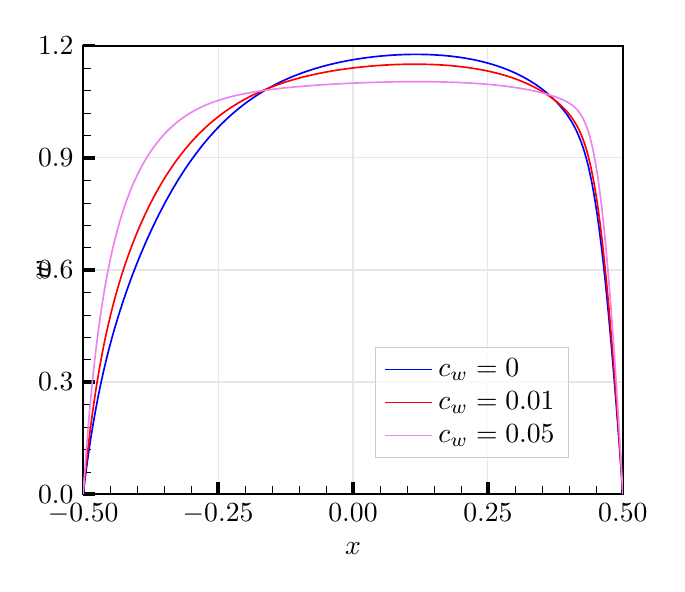
\begin{tikzpicture}

\definecolor{grey}{RGB}{128,128,128}
\definecolor{lightgrey204}{RGB}{204,204,204}
\definecolor{violet}{RGB}{238,130,238}

\begin{axis}[
legend cell align={left},
legend style={
  fill opacity=0.8,
  draw opacity=1,
  text opacity=1,
  at={(0.9,0.08)},
  anchor=south east,
  draw=lightgrey204
},
tick pos=left,
x grid style={grey!20},
xlabel={\(\displaystyle x\)},
xmajorgrids,
xmin=-0.5, xmax=0.5,
xtick style={color=black},
xtick={-0.5,-0.25,0,0.25,0.5},
xticklabels={
  \(\displaystyle {\ensuremath{-}0.50}\),
  \(\displaystyle {\ensuremath{-}0.25}\),
  \(\displaystyle {0.00}\),
  \(\displaystyle {0.25}\),
  \(\displaystyle {0.50}\)
},
y grid style={grey!20},
ylabel={\(\displaystyle w\)},
y label style={yshift=-2.5ex},
ymajorgrids,
ymin=0, ymax=1.2,
ytick style={color=black},
ytick={0,0.3,0.6,0.9,1.2},
yticklabels={
  \(\displaystyle {0.0}\),
  \(\displaystyle {0.3}\),
  \(\displaystyle {0.6}\),
  \(\displaystyle {0.9}\),
  \(\displaystyle {1.2}\)
},
minor tick num=4,
tick style={line width=1.2pt, black},
minor tick style={line width=0.15pt, black},
axis line style={line width=0.8pt, black},
]
\addplot [semithick, blue]
table {%
-0.5 0
-0.49994849945197 0.0006230607117159
-0.499794018693516 0.002488091708245
-0.499536620373079 0.0055826967515406
-0.499176408876496 0.009886405436318
-0.498713530284668 0.0153709560541192
-0.498148172314321 0.0220006871807088
-0.497480564241873 0.0297330337717139
-0.496710976810456 0.0385191202337376
-0.495839722120121 0.0483044449914014
-0.494867153501264 0.0590296416490319
-0.493793665371336 0.0706313098412411
-0.492619693074894 0.0830428937583374
-0.491345712707046 0.0961955979874534
-0.489972240920377 0.110019313999837
-0.488499834715425 0.124443543973305
-0.48692909121479 0.139398293899719
-0.485260647420981 0.154814922682823
-0.483495179958082 0.170626921792437
-0.481633404797351 0.186770615712696
-0.479676076966869 0.203185763632631
-0.477623990245336 0.219816058443311
-0.475477976840169 0.236609510911958
-0.473238907050001 0.253518721639999
-0.47090768891174 0.270501036319803
-0.468485267832324 0.287518593255239
-0.465972626205314 0.304538265785447
-0.463370783012499 0.321531513996728
-0.460680793410648 0.338474153976506
-0.457903748303608 0.355346062338618
-0.455040773899887 0.372130827244426
-0.452093031255939 0.388815364112522
-0.449061715805301 0.405389507266822
-0.445948056873795 0.421845593612104
-0.442753317180985 0.43817804747447
-0.439478792328093 0.454382979152218
-0.436125810272576 0.470457803271771
-0.432695730789584 0.486400885622159
-0.429189944920516 0.502211221495224
-0.425609874408889 0.517888150677091
-0.421956971123768 0.533431109491688
-0.418232716470968 0.548839422153745
-0.414438620792282 0.56411212982996
-0.410576222752975 0.579247857507729
-0.406647088717789 0.594244715722631
-0.402652812115718 0.609100235786137
-0.398595012793805 0.62381133480545
-0.394475336360226 0.638374308268739
-0.390295453516925 0.652784846192867
-0.386057059382078 0.667038070190022
-0.381761872802647 0.681128587487741
-0.377411635657318 0.695050559162825
-0.373008112150095 0.708797778889247
-0.368553088094842 0.722363759593927
-0.364048370191059 0.735741824741284
-0.359495785291191 0.748925201940714
-0.354897179659761 0.761907116129159
-0.350254418224633 0.774680880446013
-0.345569383820707 0.787239982657626
-0.340843976426345 0.799578165754113
-0.336080112392858 0.811689501218206
-0.331279723667337 0.82356845413255
-0.326444757009172 0.835209939260431
-0.321577173200559 0.846609367801954
-0.316678946251317 0.857762684543864
-0.311752062598348 0.868666395581421
-0.306798520300052 0.879317586820841
-0.301820328226031 0.88971393381891
-0.296819505242404 0.899853703532088
-0.291798079393078 0.909735748785119
-0.286758087077287 0.919359496252257
-0.281701572223747 0.928724928887115
-0.276630585461758 0.937832563676174
-0.271547183289587 0.946683425649516
-0.266453427240473 0.955279018992499
-0.261351383046584 0.963621296093982
-0.256243119801282 0.971712625255763
-0.251130709120015 0.979555757738553
-0.24601622430019 0.987153794701784
-0.240901739480366 0.994510154526011
-0.235789328799099 1.00162854089473
-0.230681065553797 1.00851291194236
-0.225579021359908 1.01516745068157
-0.220485265310793 1.02159653686201
-0.215401863138623 1.02780472034289
-0.210330876376634 1.0337966960179
-0.205274361523094 1.03957728028556
-0.200234369207303 1.04515138903151
-0.195212943357977 1.05052401706562
-0.19021212037435 1.0557002189469
-0.185233928300328 1.06068509112023
-0.180280386002033 1.06548375529084
-0.175353502349064 1.07010134296381
-0.170455275399822 1.07454298108358
-0.165587691591209 1.07881377871484
-0.160752724933044 1.08291881471622
-0.155952336207523 1.08686312636389
-0.151188472174036 1.09065169889162
-0.146463064779674 1.09428945591918
-0.141778030375748 1.09778125074531
-0.13713526894062 1.10113185848489
-0.13253666330919 1.1043459690317
-0.127984078409322 1.10742818082817
-0.123479360505539 1.11038299542246
-0.119024336450286 1.11321481279116
-0.114620812943063 1.1159279274037
-0.110270575797734 1.11852652500048
-0.105975389218302 1.12101468005414
-0.101736995083455 1.12339635387956
-0.097557112240155 1.12567539335516
-0.0934374358065758 1.12785553021458
-0.0893796364846631 1.12994038086605
-0.0853853598825923 1.13193344669438
-0.0814562258474062 1.13383811479888
-0.0775938278080988 1.13565765912069
-0.0737997321294127 1.13739524191134
-0.0700754774766127 1.13905391549581
-0.066422574191492 1.14063662428421
-0.0628425036798653 1.14214620698679
-0.0593367178107966 1.14358539898966
-0.0559066383278049 1.14495683485024
-0.0525536562722878 1.1462630508742
-0.0492791314193958 1.14750648773834
-0.046084391726586 1.14868949312653
-0.0429707327950797 1.14981432434902
-0.0399394173444415 1.15088315091876
-0.0369916747004938 1.15189805706103
-0.0341287002967733 1.15286104413594
-0.0313516551897324 1.1537740329567
-0.0286616655878819 1.15463886598907
-0.0260598223950666 1.15545730942049
-0.0235471807680572 1.15623105509031
-0.0211247596886407 1.15696172227458
-0.0187935415503799 1.15765085932182
-0.0165544717602116 1.15829994513813
-0.0144084583550445 1.1589103905219
-0.012356371633512 1.15948353935082
-0.0103990438030294 1.16002066962476
-0.0085372686422993 1.16052299437038
-0.0067718011794 1.16099166241383
-0.0051033573855911 1.16142775902971
-0.0035326138849561 1.16183230647475
-0.0020602076800033 1.16220626441616
-0.0006867358933344 1.16255053026352
0.0006867358933344 1.16289041304197
0.0020602076800033 1.16322593492075
0.0035326138849561 1.16358080646737
0.0051033573855911 1.16395391052467
0.0067718011794 1.16434407288205
0.0085372686422993 1.16475006562398
0.0103990438030294 1.16517061050189
0.012356371633512 1.16560438230274
0.0144084583550445 1.16605001218608
0.0165544717602116 1.16650609096303
0.0187935415503799 1.16697117229039
0.0211247596886407 1.16744377575537
0.0235471807680572 1.16792238982738
0.0260598223950666 1.16840547465502
0.0286616655878819 1.16889146468857
0.0313516551897324 1.16937877111005
0.0341287002967733 1.16986578405542
0.0369916747004938 1.17035087461585
0.0399394173444415 1.17083239660724
0.0429707327950797 1.17130868810004
0.046084391726586 1.17177807270382
0.0492791314193958 1.17223886060387
0.0525536562722878 1.1726893493495
0.0559066383278049 1.17312782439639
0.0593367178107966 1.17355255940792
0.0628425036798653 1.17396181632237
0.066422574191492 1.17435384519578
0.0700754774766127 1.17472688383168
0.0737997321294127 1.17507915721128
0.0775938278080988 1.17540887673903
0.0814562258474062 1.17571423932027
0.0853853598825923 1.1759934262886
0.0893796364846631 1.17624460220165
0.0934374358065758 1.17646591352498
0.097557112240155 1.17665548722351
0.101736995083455 1.17681142928085
0.105975389218302 1.17693182316631
0.110270575797734 1.1770147282688
0.114620812943063 1.17705817831681
0.119024336450286 1.17706017980169
0.123479360505539 1.17701871042118
0.127984078409322 1.17693171755814
0.13253666330919 1.17679711680768
0.13713526894062 1.17661279056387
0.141778030375748 1.17637658667535
0.146463064779674 1.17608631717635
0.151188472174036 1.17573975709716
0.155952336207523 1.17533464335565
0.160752724933044 1.1748686737281
0.165587691591209 1.17433950589496
0.170455275399822 1.17374475655399
0.175353502349064 1.17308200058992
0.180280386002033 1.17234877028723
0.185233928300328 1.1715425545686
0.19021212037435 1.17066079823947
0.195212943357977 1.16970090121513
0.200234369207303 1.16866021770446
0.205274361523094 1.16753605532101
0.210330876376634 1.1663256740895
0.215401863138623 1.16502628531289
0.220485265310793 1.16363505026215
0.225579021359908 1.16214907864844
0.230681065553797 1.16056542683388
0.235789328799099 1.15888109573426
0.240901739480366 1.15709302836441
0.24601622430019 1.15519810697105
0.251130709120015 1.15319314969568
0.256243119801282 1.15107490670212
0.261351383046584 1.1488400557002
0.266453427240473 1.14648519678299
0.271547183289587 1.14400684649096
0.276630585461758 1.14140143099488
0.281701572223747 1.13866527828101
0.286758087077287 1.13579460918687
0.291798079393078 1.13278552711958
0.296819505242404 1.12963400623198
0.301820328226031 1.1263358777948
0.306798520300052 1.12288681440576
0.311752062598348 1.11928231158779
0.316678946251317 1.11551766613292
0.321577173200559 1.11158795032568
0.326444757009172 1.10748798071906
0.331279723667337 1.10321227950844
0.336080112392858 1.09875502538969
0.340843976426345 1.09410998908057
0.345569383820707 1.08927044583847
0.350254418224633 1.0842290532455
0.354897179659761 1.07897767652355
0.359495785291191 1.0735071359435
0.364048370191059 1.06780684131826
0.368553088094842 1.06186426883121
0.373008112150095 1.05566422725781
0.377411635657318 1.04918785853398
0.381761872802647 1.04241132579016
0.386057059382078 1.03530416692912
0.390295453516925 1.0278273369169
0.394475336360226 1.01993102984074
0.398595012793805 1.01155245694129
0.402652812115718 1.00261385008589
0.406647088717789 0.993021041769088
0.410576222752975 0.982663022720837
0.414438620792282 0.971412871675986
0.418232716470968 0.959130375843505
0.421956971123768 0.945666507611926
0.425609874408889 0.93086970948494
0.429189944920516 0.914593688717895
0.432695730789584 0.896706182070814
0.436125810272576 0.877097957133955
0.439478792328093 0.855691216744909
0.442753317180985 0.832446580985412
0.445948056873795 0.807367951593731
0.449061715805301 0.780504783848082
0.452093031255939 0.751951580898025
0.455040773899887 0.721844720485826
0.457903748303608 0.690357000286338
0.460680793410648 0.657690483568144
0.463370783012499 0.624068348643071
0.465972626205314 0.589726455618105
0.468485267832324 0.554905289970101
0.47090768891174 0.51984280416579
0.473238907050001 0.484768529016773
0.475477976840169 0.449899141323993
0.477623990245336 0.415435531507185
0.479676076966869 0.381561269121328
0.481633404797351 0.34844228833703
0.483495179958082 0.316227540943301
0.485260647420981 0.28505036164958
0.48692909121479 0.255030274226922
0.488499834715425 0.226275012303887
0.489972240920377 0.198882541557158
0.491345712707046 0.172942934707114
0.492619693074894 0.148539968887643
0.493793665371336 0.125752380330645
0.494867153501264 0.104654722394563
0.495839722120121 0.0853178310450246
0.496710976810456 0.0678089026287389
0.497480564241873 0.0521912375262646
0.498148172314321 0.0385236948442826
0.498713530284668 0.0268599413454649
0.499176408876496 0.0172475637259045
0.499536620373079 0.0097271355206734
0.499794018693516 0.0043313160331238
0.49994849945197 0.0010840596297053
0.5 0
};
\addlegendentry{\(\displaystyle c_w=0\)}
\addplot [semithick, red]
table {%
-0.5 0
-0.49994849945197 0.0007757778852536
-0.499794018693516 0.0030975358773917
-0.499536620373079 0.0069486219633345
-0.499176408876496 0.0123015320479077
-0.498713530284668 0.0191182814872202
-0.498148172314321 0.0273509202911129
-0.497480564241873 0.0369421872383088
-0.496710976810456 0.0478262940993962
-0.495839722120121 0.0599298334749876
-0.494867153501264 0.0731727920235325
-0.493793665371336 0.0874696599977893
-0.492619693074894 0.102730609126389
-0.491345712707046 0.118862724230309
-0.489972240920377 0.135771253674271
-0.488499834715425 0.153360859343514
-0.48692909121479 0.171536828903876
-0.485260647420981 0.190206230828317
-0.483495179958082 0.209278978420165
-0.481633404797351 0.228668788167785
-0.479676076966869 0.248294006620277
-0.477623990245336 0.268078299009128
-0.475477976840169 0.287951183780768
-0.473238907050001 0.307848415202127
-0.47090768891174 0.327712208716504
-0.468485267832324 0.34749132020935
-0.465972626205314 0.367140983877831
-0.463370783012499 0.386622727595841
-0.460680793410648 0.405904078208249
-0.457903748303608 0.424958180210326
-0.455040773899887 0.443763344036314
-0.452093031255939 0.462302547823673
-0.449061715805301 0.480562908563715
-0.445948056873795 0.498535143450892
-0.442753317180985 0.516213034197251
-0.439478792328093 0.533592910193164
-0.436125810272576 0.550673158920575
-0.432695730789584 0.567453774150844
-0.429189944920516 0.583935945965428
-0.425609874408889 0.600121698294729
-0.421956971123768 0.616013574321925
-0.418232716470968 0.631614371584156
-0.414438620792282 0.646926924398889
-0.410576222752975 0.661953932699085
-0.406647088717789 0.67669783319185
-0.402652812115718 0.691160710217018
-0.398595012793805 0.705344241380807
-0.394475336360226 0.719249674480638
-0.390295453516925 0.73287783061989
-0.386057059382078 0.746229129788723
-0.381761872802647 0.759303634083859
-0.377411635657318 0.772101105015288
-0.373008112150095 0.784621070628894
-0.368553088094842 0.796862899325056
-0.364048370191059 0.808825876815519
-0.359495785291191 0.820509283684452
-0.354897179659761 0.831912470785911
-0.350254418224633 0.843034930607544
-0.345569383820707 0.853876362641059
-0.340843976426345 0.864436731573976
-0.336080112392858 0.874716317120758
-0.331279723667337 0.884715754963282
-0.326444757009172 0.894436068321177
-0.321577173200559 0.903878690202441
-0.316678946251317 0.913045476444744
-0.311752062598348 0.92193871006397
-0.306798520300052 0.930561097467348
-0.301820328226031 0.938915757373584
-0.296819505242404 0.94700620328583
-0.291798079393078 0.954836320534094
-0.286758087077287 0.962410338862455
-0.281701572223747 0.969732801612608
-0.276630585461758 0.97680853246709
-0.271547183289587 0.983642600714524
-0.266453427240473 0.990240285882209
-0.261351383046584 0.996607042525449
-0.256243119801282 1.00274846582992
-0.251130709120015 1.00867025859752
-0.24601622430019 1.01437820005399
-0.240901739480366 1.01987811682312
-0.235789328799099 1.02517585629321
-0.230681065553797 1.03027726251789
-0.225579021359908 1.03518815469806
-0.220485265310793 1.0399143082258
-0.215401863138623 1.04446143820586
-0.210330876376634 1.04883518532668
-0.205274361523094 1.05304110391563
-0.200234369207303 1.05708465199196
-0.195212943357977 1.06097118311722
-0.19021212037435 1.06470593984046
-0.185233928300328 1.06829404853868
-0.180280386002033 1.0717405154637
-0.175353502349064 1.07505022381979
-0.170455275399822 1.07822793171389
-0.165587691591209 1.08127827083874
-0.160752724933044 1.08420574576859
-0.155952336207523 1.0870147337645
-0.151188472174036 1.08970948500488
-0.146463064779674 1.09229412317252
-0.141778030375748 1.09477264634266
-0.13713526894062 1.0971489281291
-0.13253666330919 1.09942671905489
-0.127984078409322 1.10160964812186
-0.123479360505539 1.10370122455923
-0.119024336450286 1.10570483973541
-0.114620812943063 1.1076237692203
-0.110270575797734 1.10946117498674
-0.105975389218302 1.11122010774046
-0.101736995083455 1.11290350936806
-0.097557112240155 1.11451421549161
-0.0934374358065758 1.11605495811813
-0.0893796364846631 1.11752836837106
-0.0853853598825923 1.11893697928959
-0.0814562258474062 1.12028322868134
-0.0775938278080988 1.12156946201299
-0.0737997321294127 1.12279793532252
-0.0700754774766127 1.12397081813692
-0.066422574191492 1.12509019637916
-0.0628425036798653 1.12615807524829
-0.0593367178107966 1.12717638205673
-0.0559066383278049 1.12814696901006
-0.0525536562722878 1.12907161591507
-0.0492791314193958 1.12995203280312
-0.046084391726586 1.13078986245672
-0.0429707327950797 1.13158668282884
-0.0399394173444415 1.13234400934582
-0.0369916747004938 1.133063297086
-0.0341287002967733 1.13374594282762
-0.0313516551897324 1.13439328696152
-0.0286616655878819 1.13500661526484
-0.0260598223950666 1.13558716053397
-0.0235471807680572 1.13613610407621
-0.0211247596886407 1.13665457706078
-0.0187935415503799 1.13714366173119
-0.0165544717602116 1.13760439248226
-0.0144084583550445 1.13803775680581
-0.012356371633512 1.1384446961103
-0.0103990438030294 1.13882610642061
-0.0085372686422993 1.13918283896462
-0.0067718011794 1.13951570065425
-0.0051033573855911 1.13982545446884
-0.0035326138849561 1.14011281974945
-0.0020602076800033 1.14037847241295
-0.0006867358933344 1.14062304509415
0.0006867358933344 1.14086451485416
0.0020602076800033 1.14110289591247
0.0035326138849561 1.14135503342147
0.0051033573855911 1.14162013339671
0.0067718011794 1.14189736055346
0.0085372686422993 1.14218584054098
0.0103990438030294 1.1424846621861
0.012356371633512 1.14279287972777
0.0144084583550445 1.14310951502329
0.0165544717602116 1.143433559708
0.0187935415503799 1.14376397729046
0.0211247596886407 1.14409970516644
0.0235471807680572 1.14443965653574
0.0260598223950666 1.14478272220749
0.0286616655878819 1.14512777228052
0.0313516551897324 1.14547365768732
0.0341287002967733 1.14581921159125
0.0369916747004938 1.14616325062859
0.0399394173444415 1.14650457598863
0.0429707327950797 1.14684197432691
0.046084391726586 1.14717421850807
0.0492791314193958 1.14750006817718
0.0525536562722878 1.14781827015975
0.0559066383278049 1.14812755869242
0.0593367178107966 1.14842665548812
0.0628425036798653 1.14871426964065
0.066422574191492 1.14898909737596
0.0700754774766127 1.1492498216578
0.0737997321294127 1.14949511165744
0.0775938278080988 1.14972362209783
0.0814562258474062 1.1499339924836
0.0853853598825923 1.15012484622944
0.0893796364846631 1.15029478969936
0.0934374358065758 1.15044241117064
0.097557112240155 1.15056627973567
0.101736995083455 1.1506649441557
0.105975389218302 1.15073693168001
0.110270575797734 1.15078074684377
0.114620812943063 1.15079487025737
0.119024336450286 1.15077775739944
0.123479360505539 1.15072783742498
0.127984078409322 1.1506435119986
0.13253666330919 1.15052315416212
0.13713526894062 1.15036510724389
0.141778030375748 1.15016768381632
0.146463064779674 1.14992916470569
0.151188472174036 1.14964779805688
0.155952336207523 1.14932179845392
0.160752724933044 1.14894934609453
0.165587691591209 1.14852858601538
0.170455275399822 1.14805762736221
0.175353502349064 1.14753454269651
0.180280386002033 1.14695736732862
0.185233928300328 1.14632409866444
0.19021212037435 1.14563269555059
0.195212943357977 1.14488107760057
0.200234369207303 1.14406712448218
0.205274361523094 1.1431886751441
0.210330876376634 1.14224352695729
0.215401863138623 1.14122943474457
0.220485265310793 1.14014410966927
0.225579021359908 1.13898521795175
0.230681065553797 1.13775037937991
0.235789328799099 1.13643716557725
0.240901739480366 1.13504309798963
0.24601622430019 1.13356564554733
0.251130709120015 1.13200222195673
0.256243119801282 1.13035018256936
0.261351383046584 1.1286068207733
0.266453427240473 1.12676936384116
0.271547183289587 1.12483496816358
0.276630585461758 1.1228007137821
0.281701572223747 1.12066359812585
0.286758087077287 1.11842052883003
0.291798079393078 1.11606831549925
0.296819505242404 1.11360366023392
0.301820328226031 1.111023146706
0.306798520300052 1.1083232274916
0.311752062598348 1.10550020929078
0.316678946251317 1.10255023549885
0.321577173200559 1.09946926539118
0.326444757009172 1.09625304876567
0.331279723667337 1.09289709428532
0.336080112392858 1.0893966286415
0.340843976426345 1.08574654193362
0.345569383820707 1.0819413117531
0.350254418224633 1.07797489415551
0.354897179659761 1.07384056325103
0.359495785291191 1.06953067256249
0.364048370191059 1.06503630036481
0.368553088094842 1.06034672938717
0.373008112150095 1.05544870036291
0.377411635657318 1.05032537349675
0.381761872802647 1.04495493683713
0.386057059382078 1.03930882292984
0.390295453516925 1.03334953975712
0.394475336360226 1.02702819254297
0.398595012793805 1.02028186551683
0.402652812115718 1.01303113819463
0.406647088717789 1.00517810933324
0.410576222752975 0.99660537108339
0.414438620792282 0.987176388416998
0.418232716470968 0.976737676893036
0.421956971123768 0.965123024242727
0.425609874408889 0.952159780577041
0.429189944920516 0.937676971550437
0.432695730789584 0.921514715586795
0.436125810272576 0.903534193209863
0.439478792328093 0.883627275595879
0.442753317180985 0.861724892728967
0.445948056873795 0.837803328257266
0.449061715805301 0.811887841223864
0.452093031255939 0.784053313718139
0.455040773899887 0.754421942997867
0.457903748303608 0.723158307080607
0.460680793410648 0.690462367638541
0.463370783012499 0.656561132912551
0.465972626205314 0.621699744523838
0.468485267832324 0.586132718709789
0.47090768891174 0.550115944106001
0.473238907050001 0.513899887712761
0.475477976840169 0.477724266337762
0.477623990245336 0.44181428320002
0.479676076966869 0.406378366188694
0.481633404797351 0.371607251603568
0.483495179958082 0.337674167389168
0.485260647420981 0.304735855768481
0.48692909121479 0.272934150091542
0.488499834715425 0.242397861561063
0.489972240920377 0.213244741229605
0.491345712707046 0.185583347864016
0.492619693074894 0.159514670741837
0.493793665371336 0.135133425329322
0.494867153501264 0.112528953099678
0.495839722120121 0.0917857197995931
0.496710976810456 0.072983409890574
0.497480564241873 0.0561966684720967
0.498148172314321 0.0414945354120023
0.498713530284668 0.0289396580168703
0.499176408876496 0.0185873551047846
0.499536620373079 0.0104846294526914
0.499794018693516 0.0046692115536309
0.49994849945197 0.0011687188331739
0.5 0
};
\addlegendentry{\(\displaystyle c_w=0.01\)}
\addplot [semithick, violet]
table {%
-0.5 0
-0.49994849945197 0.0011129310193128
-0.499794018693516 0.0044426873079972
-0.499536620373079 0.0099622779927262
-0.499176408876496 0.017627115797779
-0.498713530284668 0.0273756110692171
-0.498148172314321 0.0391299982528427
-0.497480564241873 0.0527973892060262
-0.496710976810456 0.0682710416223167
-0.495839722120121 0.0854318330618087
-0.494867153501264 0.104149913936509
-0.493793665371336 0.124286523900429
-0.492619693074894 0.145695929131473
-0.491345712707046 0.168227454728658
-0.489972240920377 0.191727557788402
-0.488499834715425 0.216041906535465
-0.48692909121479 0.241017405816465
-0.485260647420981 0.266504132246446
-0.483495179958082 0.292357123152605
-0.481633404797351 0.31843798925447
-0.479676076966869 0.344616307754896
-0.477623990245336 0.370770779540333
-0.475477976840169 0.396790125273078
-0.473238907050001 0.422573721328792
-0.47090768891174 0.448031970070933
-0.468485267832324 0.473086422378523
-0.465972626205314 0.497669664537688
-0.463370783012499 0.521725000704961
-0.460680793410648 0.545205955438598
-0.457903748303608 0.568075634548772
-0.455040773899887 0.590305974057934
-0.452093031255939 0.611876915523692
-0.449061715805301 0.63277553602699
-0.445948056873795 0.652995165427266
-0.442753317180985 0.672534513087165
-0.439478792328093 0.691396827993792
-0.436125810272576 0.709589106484046
-0.432695730789584 0.727121362313499
-0.429189944920516 0.744005965528354
-0.425609874408889 0.760257056850497
-0.421956971123768 0.775890037763736
-0.418232716470968 0.790921136932811
-0.414438620792282 0.805367048810771
-0.410576222752975 0.819244641090898
-0.406647088717789 0.832570724409535
-0.402652812115718 0.845361878833628
-0.398595012793805 0.857634329625071
-0.394475336360226 0.869403866103048
-0.390295453516925 0.880685796260492
-0.386057059382078 0.891494931182509
-0.381761872802647 0.901845592738709
-0.377411635657318 0.91175163936154
-0.373008112150095 0.921226504522025
-0.368553088094842 0.930283243732006
-0.364048370191059 0.938934585923393
-0.359495785291191 0.947192986118259
-0.354897179659761 0.95507067644553
-0.350254418224633 0.962579713459805
-0.345569383820707 0.969732019912982
-0.340843976426345 0.976539419867729
-0.336080112392858 0.983013666245098
-0.331279723667337 0.989166460482183
-0.326444757009172 0.995009464154023
-0.321577173200559 1.00055430285273
-0.316678946251317 1.00581256274796
-0.311752062598348 1.01079578055632
-0.306798520300052 1.01551542771859
-0.301820328226031 1.0199828897652
-0.296819505242404 1.02420944185768
-0.291798079393078 1.0282062215705
-0.286758087077287 1.03198419992603
-0.281701572223747 1.03555415168945
-0.276630585461758 1.03892662583122
-0.271547183289587 1.04211191699777
-0.266453427240473 1.04512003870506
-0.261351383046584 1.04796069886699
-0.256243119801282 1.05064327813287
-0.251130709120015 1.05317681139463
-0.24601622430019 1.0555699726936
-0.240901739480366 1.05783106364954
-0.235789328799099 1.05996800542362
-0.230681065553797 1.06198833414081
-0.225579021359908 1.0638991996139
-0.220485265310793 1.06570736715122
-0.215401863138623 1.06741922217871
-0.210330876376634 1.0690407773738
-0.205274361523094 1.07057768198671
-0.200234369207303 1.07203523301516
-0.195212943357977 1.07341838790075
-0.19021212037435 1.07473177842488
-0.185233928300328 1.0759797254989
-0.180280386002033 1.0771662545674
-0.175353502349064 1.0782951113687
-0.170455275399822 1.07936977782569
-0.165587691591209 1.08039348787108
-0.160752724933044 1.08136924303958
-0.155952336207523 1.08229982768887
-0.151188472174036 1.08318782373853
-0.146463064779674 1.08403562484124
-0.141778030375748 1.08484544992246
-0.13713526894062 1.08561935604529
-0.13253666330919 1.08635925057425
-0.127984078409322 1.08706690262647
-0.123479360505539 1.08774395381046
-0.119024336450286 1.08839192826294
-0.114620812943063 1.08901224200126
-0.110270575797734 1.08960621161562
-0.105975389218302 1.09017506232822
-0.101736995083455 1.09071993545092
-0.097557112240155 1.09124189527307
-0.0934374358065758 1.09174193541283
-0.0893796364846631 1.09222098466534
-0.0853853598825923 1.09267991237993
-0.0814562258474062 1.09311953339773
-0.0775938278080988 1.09354061258058
-0.0737997321294127 1.09394386895883
-0.0700754774766127 1.09432997952587
-0.066422574191492 1.09469958270418
-0.0628425036798653 1.09505328150678
-0.0593367178107966 1.09539164641558
-0.0559066383278049 1.0957152179972
-0.0525536562722878 1.096024509275
-0.0492791314193958 1.09632000787468
-0.046084391726586 1.09660217795937
-0.0429707327950797 1.09687146196928
-0.0399394173444415 1.09712828217958
-0.0369916747004938 1.09737304208938
-0.0341287002967733 1.09760612765369
-0.0313516551897324 1.09782790836976
-0.0286616655878819 1.09803873822799
-0.0260598223950666 1.09823895653764
-0.0235471807680572 1.09842888863638
-0.0211247596886407 1.09860884649294
-0.0187935415503799 1.09877912921112
-0.0165544717602116 1.09894002344328
-0.0144084583550445 1.09909180372138
-0.012356371633512 1.09923473271286
-0.0103990438030294 1.09936906140863
-0.0085372686422993 1.09949502925038
-0.0067718011794 1.09961286420371
-0.0051033573855911 1.09972278278395
-0.0035326138849561 1.0998249900407
-0.0020602076800033 1.0999196795074
-0.0006867358933344 1.10000703312212
0.0006867358933344 1.1000934495064
0.0020602076800033 1.1001789308364
0.0035326138849561 1.10026953338799
0.0051033573855911 1.10036500752616
0.0067718011794 1.10046508946354
0.0085372686422993 1.10056950173517
0.0103990438030294 1.10067795366527
0.012356371633512 1.10079014182076
0.0144084583550445 1.10090575044649
0.0165544717602116 1.10102445187807
0.0187935415503799 1.10114590692781
0.0211247596886407 1.10126976523997
0.0235471807680572 1.1013956656119
0.0260598223950666 1.10152323627807
0.0286616655878819 1.10165209515437
0.0313516551897324 1.10178185004074
0.0341287002967733 1.10191209878024
0.0369916747004938 1.10204242937374
0.0399394173444415 1.10217242004919
0.0429707327950797 1.10230163928546
0.046084391726586 1.10242964579091
0.0492791314193958 1.10255598843722
0.0525536562722878 1.10268020614972
0.0559066383278049 1.10280182775565
0.0593367178107966 1.10292037179187
0.0628425036798653 1.10303534627453
0.066422574191492 1.10314624843283
0.0700754774766127 1.1032525644098
0.0737997321294127 1.10335376893292
0.0775938278080988 1.10344932495795
0.0814562258474062 1.10353868328901
0.0853853598825923 1.10362128217887
0.0893796364846631 1.10369654691242
0.0934374358065758 1.10376388937782
0.097557112240155 1.10382270762825
0.101736995083455 1.10387238543862
0.105975389218302 1.10391229186067
0.110270575797734 1.10394178077986
0.114620812943063 1.1039601904779
0.119024336450286 1.10396684320402
0.123479360505539 1.1039610447579
0.127984078409322 1.10394208408753
0.13253666330919 1.10390923290396
0.13713526894062 1.1038617453153
0.141778030375748 1.10379885748162
0.146463064779674 1.10371978729189
0.151188472174036 1.10362373406343
0.155952336207523 1.10350987826428
0.160752724933044 1.10337738125734
0.165587691591209 1.10322538506545
0.170455275399822 1.10305301215495
0.175353502349064 1.10285936523484
0.180280386002033 1.10264352706794
0.185233928300328 1.10240456028952
0.19021212037435 1.10214150722732
0.195212943357977 1.10185338971688
0.200234369207303 1.10153920890475
0.205274361523094 1.10119794503044
0.210330876376634 1.10082855717841
0.215401863138623 1.10042998298903
0.220485265310793 1.10000113831648
0.225579021359908 1.09954091682153
0.230681065553797 1.09904818948426
0.235789328799099 1.09852180402204
0.240901739480366 1.09796058419552
0.24601622430019 1.09736332898407
0.251130709120015 1.0967288116107
0.256243119801282 1.09605577839293
0.261351383046584 1.09534294739593
0.266453427240473 1.0945890068577
0.271547183289587 1.09379261335488
0.276630585461758 1.09295238967028
0.281701572223747 1.09206692231952
0.286758087077287 1.0911347586819
0.291798079393078 1.09015440367355
0.296819505242404 1.08912431588172
0.301820328226031 1.08804290306122
0.306798520300052 1.08690851685566
0.311752062598348 1.08571944656007
0.316678946251317 1.08447391163985
0.321577173200559 1.08317005256814
0.326444757009172 1.08180591922574
0.331279723667337 1.08037945556486
0.336080112392858 1.07888847820647
0.340843976426345 1.07733064487953
0.345569383820707 1.07570340556975
0.350254418224633 1.07400392441074
0.354897179659761 1.07222895290044
0.359495785291191 1.07037462447784
0.364048370191059 1.06843612649418
0.368553088094842 1.06640718906409
0.373008112150095 1.06427931323529
0.377411635657318 1.06204064793504
0.381761872802647 1.0596744225156
0.386057059382078 1.05715685797803
0.390295453516925 1.05445452303912
0.394475336360226 1.0515211773078
0.398595012793805 1.04829425238878
0.402652812115718 1.04469125442917
0.406647088717789 1.04060650859757
0.410576222752975 1.03590877981789
0.414438620792282 1.03044036110701
0.418232716470968 1.02401819261406
0.421956971123768 1.0164374415885
0.425609874408889 1.00747773920931
0.429189944920516 0.99691195647299
0.432695730789584 0.984517056139318
0.436125810272576 0.970086235414178
0.439478792328093 0.953441338141538
0.442753317180985 0.934444406377461
0.445948056873795 0.913007290274683
0.449061715805301 0.889098427876057
0.452093031255939 0.862746222259418
0.455040773899887 0.834038816468322
0.457903748303608 0.803120454145563
0.460680793410648 0.770184938833289
0.463370783012499 0.735466950296029
0.465972626205314 0.699232090929717
0.468485267832324 0.661766552242945
0.47090768891174 0.623367188660345
0.473238907050001 0.584332636207338
0.475477976840169 0.544955900475522
0.477623990245336 0.505518648422139
0.479676076966869 0.466287235754602
0.481633404797351 0.427510369507302
0.483495179958082 0.38941817844534
0.485260647420981 0.352222421356758
0.48692909121479 0.316117515444255
0.488499834715425 0.281282096340535
0.489972240920377 0.247880823398808
0.491345712707046 0.216066211387716
0.492619693074894 0.185980290246684
0.493793665371336 0.157755972900998
0.494867153501264 0.131518029869598
0.495839722120121 0.107383643687388
0.496710976810456 0.0854625246943507
0.497480564241873 0.0658566338109533
0.498148172314321 0.0486595549541192
0.498713530284668 0.0339556099386371
0.499176408876496 0.0218187969970529
0.499536620373079 0.0123116634153077
0.499794018693516 0.0054842087221517
0.49994849945197 0.0013729169241406
0.5 0
};
\addlegendentry{\(\displaystyle c_w=0.05\)}
\end{axis}
\end{tikzpicture}
}
		\label{fig:phv}}
\end{figure}

\begin{lstlisting}[numbers=left,frame=single,language=Python]
\begin{tikzpicture}

\definecolor{grey}{RGB}{128,128,128}
\definecolor{lightgrey204}{RGB}{204,204,204}
\definecolor{violet}{RGB}{238,130,238}

\begin{axis}[
legend cell align={left},
legend style={
fill opacity=0.8,
draw opacity=1,
text opacity=1,
at={(0.9,0.08)},
anchor=south east,
draw=lightgrey204
},
tick pos=left,
x grid style={grey!20},
xlabel={\(\displaystyle x\)},
xmajorgrids,
xmin=-0.5, xmax=0.5,
xtick style={color=black},
xtick={-0.5,-0.25,0,0.25,0.5},
xticklabels={
\(\displaystyle {\ensuremath{-}0.50}\),
\(\displaystyle {\ensuremath{-}0.25}\),
\(\displaystyle {0.00}\),
\(\displaystyle {0.25}\),
\(\displaystyle {0.50}\)
},
y grid style={grey!20},
ylabel={\(\displaystyle w\)},
y label style={yshift=-2.5ex},
ymajorgrids,
ymin=0, ymax=1.2,
ytick style={color=black},
ytick={0,0.3,0.6,0.9,1.2},
yticklabels={
\(\displaystyle {0.0}\),
\(\displaystyle {0.3}\),
\(\displaystyle {0.6}\),
\(\displaystyle {0.9}\),
\(\displaystyle {1.2}\)
},
minor tick num=4,
tick style={line width=1.2pt, black},
minor tick style={line width=0.15pt, black},
axis line style={line width=0.8pt, black},
]
\addplot [semithick, blue]
table {%
...
};
\addlegendentry{\(\displaystyle c_w=0.05\)}
\end{axis}
\end{tikzpicture}
\end{lstlisting}

其中第33,45,46,47,48行都是后来手动加上去的,第13行position也有有调整;33行平移轴线位置,45行设置副刻度数量,46-47设置主副刻度线粗细,48设置轴线粗细;\par

在文中的插入只需用\verb input 命令对外部的tex文件进行插入即可,例如上文中对图片的插入:\par

\begin{lstlisting}[numbers=left,frame=single,language=Python]
\begin{figure}[htbp]
  \centering{
  \raisebox{33ex}{\makebox[0pt][l]{(a)}}
  \scalebox{0.78}{% This file was created with tikzplotlib v0.10.1.post12.
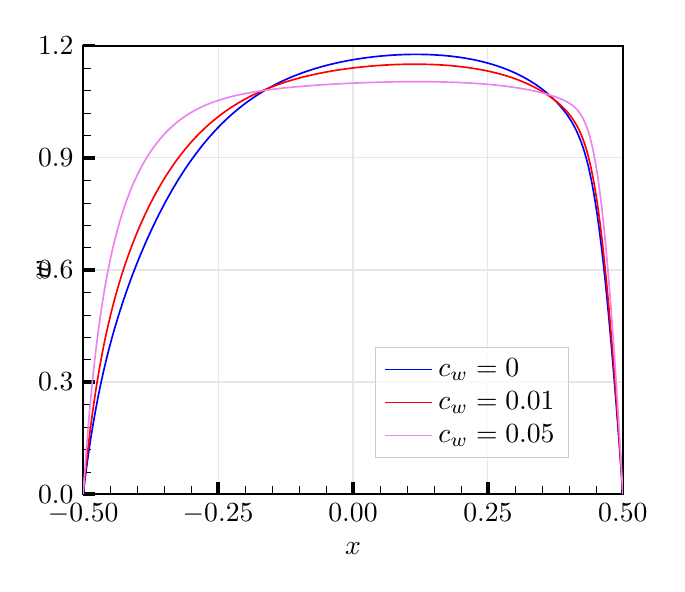
\begin{tikzpicture}

\definecolor{grey}{RGB}{128,128,128}
\definecolor{lightgrey204}{RGB}{204,204,204}
\definecolor{violet}{RGB}{238,130,238}

\begin{axis}[
legend cell align={left},
legend style={
  fill opacity=0.8,
  draw opacity=1,
  text opacity=1,
  at={(0.9,0.08)},
  anchor=south east,
  draw=lightgrey204
},
tick pos=left,
x grid style={grey!20},
xlabel={\(\displaystyle x\)},
xmajorgrids,
xmin=-0.5, xmax=0.5,
xtick style={color=black},
xtick={-0.5,-0.25,0,0.25,0.5},
xticklabels={
  \(\displaystyle {\ensuremath{-}0.50}\),
  \(\displaystyle {\ensuremath{-}0.25}\),
  \(\displaystyle {0.00}\),
  \(\displaystyle {0.25}\),
  \(\displaystyle {0.50}\)
},
y grid style={grey!20},
ylabel={\(\displaystyle w\)},
y label style={yshift=-2.5ex},
ymajorgrids,
ymin=0, ymax=1.2,
ytick style={color=black},
ytick={0,0.3,0.6,0.9,1.2},
yticklabels={
  \(\displaystyle {0.0}\),
  \(\displaystyle {0.3}\),
  \(\displaystyle {0.6}\),
  \(\displaystyle {0.9}\),
  \(\displaystyle {1.2}\)
},
minor tick num=4,
tick style={line width=1.2pt, black},
minor tick style={line width=0.15pt, black},
axis line style={line width=0.8pt, black},
]
\addplot [semithick, blue]
table {%
-0.5 0
-0.49994849945197 0.0006230607117159
-0.499794018693516 0.002488091708245
-0.499536620373079 0.0055826967515406
-0.499176408876496 0.009886405436318
-0.498713530284668 0.0153709560541192
-0.498148172314321 0.0220006871807088
-0.497480564241873 0.0297330337717139
-0.496710976810456 0.0385191202337376
-0.495839722120121 0.0483044449914014
-0.494867153501264 0.0590296416490319
-0.493793665371336 0.0706313098412411
-0.492619693074894 0.0830428937583374
-0.491345712707046 0.0961955979874534
-0.489972240920377 0.110019313999837
-0.488499834715425 0.124443543973305
-0.48692909121479 0.139398293899719
-0.485260647420981 0.154814922682823
-0.483495179958082 0.170626921792437
-0.481633404797351 0.186770615712696
-0.479676076966869 0.203185763632631
-0.477623990245336 0.219816058443311
-0.475477976840169 0.236609510911958
-0.473238907050001 0.253518721639999
-0.47090768891174 0.270501036319803
-0.468485267832324 0.287518593255239
-0.465972626205314 0.304538265785447
-0.463370783012499 0.321531513996728
-0.460680793410648 0.338474153976506
-0.457903748303608 0.355346062338618
-0.455040773899887 0.372130827244426
-0.452093031255939 0.388815364112522
-0.449061715805301 0.405389507266822
-0.445948056873795 0.421845593612104
-0.442753317180985 0.43817804747447
-0.439478792328093 0.454382979152218
-0.436125810272576 0.470457803271771
-0.432695730789584 0.486400885622159
-0.429189944920516 0.502211221495224
-0.425609874408889 0.517888150677091
-0.421956971123768 0.533431109491688
-0.418232716470968 0.548839422153745
-0.414438620792282 0.56411212982996
-0.410576222752975 0.579247857507729
-0.406647088717789 0.594244715722631
-0.402652812115718 0.609100235786137
-0.398595012793805 0.62381133480545
-0.394475336360226 0.638374308268739
-0.390295453516925 0.652784846192867
-0.386057059382078 0.667038070190022
-0.381761872802647 0.681128587487741
-0.377411635657318 0.695050559162825
-0.373008112150095 0.708797778889247
-0.368553088094842 0.722363759593927
-0.364048370191059 0.735741824741284
-0.359495785291191 0.748925201940714
-0.354897179659761 0.761907116129159
-0.350254418224633 0.774680880446013
-0.345569383820707 0.787239982657626
-0.340843976426345 0.799578165754113
-0.336080112392858 0.811689501218206
-0.331279723667337 0.82356845413255
-0.326444757009172 0.835209939260431
-0.321577173200559 0.846609367801954
-0.316678946251317 0.857762684543864
-0.311752062598348 0.868666395581421
-0.306798520300052 0.879317586820841
-0.301820328226031 0.88971393381891
-0.296819505242404 0.899853703532088
-0.291798079393078 0.909735748785119
-0.286758087077287 0.919359496252257
-0.281701572223747 0.928724928887115
-0.276630585461758 0.937832563676174
-0.271547183289587 0.946683425649516
-0.266453427240473 0.955279018992499
-0.261351383046584 0.963621296093982
-0.256243119801282 0.971712625255763
-0.251130709120015 0.979555757738553
-0.24601622430019 0.987153794701784
-0.240901739480366 0.994510154526011
-0.235789328799099 1.00162854089473
-0.230681065553797 1.00851291194236
-0.225579021359908 1.01516745068157
-0.220485265310793 1.02159653686201
-0.215401863138623 1.02780472034289
-0.210330876376634 1.0337966960179
-0.205274361523094 1.03957728028556
-0.200234369207303 1.04515138903151
-0.195212943357977 1.05052401706562
-0.19021212037435 1.0557002189469
-0.185233928300328 1.06068509112023
-0.180280386002033 1.06548375529084
-0.175353502349064 1.07010134296381
-0.170455275399822 1.07454298108358
-0.165587691591209 1.07881377871484
-0.160752724933044 1.08291881471622
-0.155952336207523 1.08686312636389
-0.151188472174036 1.09065169889162
-0.146463064779674 1.09428945591918
-0.141778030375748 1.09778125074531
-0.13713526894062 1.10113185848489
-0.13253666330919 1.1043459690317
-0.127984078409322 1.10742818082817
-0.123479360505539 1.11038299542246
-0.119024336450286 1.11321481279116
-0.114620812943063 1.1159279274037
-0.110270575797734 1.11852652500048
-0.105975389218302 1.12101468005414
-0.101736995083455 1.12339635387956
-0.097557112240155 1.12567539335516
-0.0934374358065758 1.12785553021458
-0.0893796364846631 1.12994038086605
-0.0853853598825923 1.13193344669438
-0.0814562258474062 1.13383811479888
-0.0775938278080988 1.13565765912069
-0.0737997321294127 1.13739524191134
-0.0700754774766127 1.13905391549581
-0.066422574191492 1.14063662428421
-0.0628425036798653 1.14214620698679
-0.0593367178107966 1.14358539898966
-0.0559066383278049 1.14495683485024
-0.0525536562722878 1.1462630508742
-0.0492791314193958 1.14750648773834
-0.046084391726586 1.14868949312653
-0.0429707327950797 1.14981432434902
-0.0399394173444415 1.15088315091876
-0.0369916747004938 1.15189805706103
-0.0341287002967733 1.15286104413594
-0.0313516551897324 1.1537740329567
-0.0286616655878819 1.15463886598907
-0.0260598223950666 1.15545730942049
-0.0235471807680572 1.15623105509031
-0.0211247596886407 1.15696172227458
-0.0187935415503799 1.15765085932182
-0.0165544717602116 1.15829994513813
-0.0144084583550445 1.1589103905219
-0.012356371633512 1.15948353935082
-0.0103990438030294 1.16002066962476
-0.0085372686422993 1.16052299437038
-0.0067718011794 1.16099166241383
-0.0051033573855911 1.16142775902971
-0.0035326138849561 1.16183230647475
-0.0020602076800033 1.16220626441616
-0.0006867358933344 1.16255053026352
0.0006867358933344 1.16289041304197
0.0020602076800033 1.16322593492075
0.0035326138849561 1.16358080646737
0.0051033573855911 1.16395391052467
0.0067718011794 1.16434407288205
0.0085372686422993 1.16475006562398
0.0103990438030294 1.16517061050189
0.012356371633512 1.16560438230274
0.0144084583550445 1.16605001218608
0.0165544717602116 1.16650609096303
0.0187935415503799 1.16697117229039
0.0211247596886407 1.16744377575537
0.0235471807680572 1.16792238982738
0.0260598223950666 1.16840547465502
0.0286616655878819 1.16889146468857
0.0313516551897324 1.16937877111005
0.0341287002967733 1.16986578405542
0.0369916747004938 1.17035087461585
0.0399394173444415 1.17083239660724
0.0429707327950797 1.17130868810004
0.046084391726586 1.17177807270382
0.0492791314193958 1.17223886060387
0.0525536562722878 1.1726893493495
0.0559066383278049 1.17312782439639
0.0593367178107966 1.17355255940792
0.0628425036798653 1.17396181632237
0.066422574191492 1.17435384519578
0.0700754774766127 1.17472688383168
0.0737997321294127 1.17507915721128
0.0775938278080988 1.17540887673903
0.0814562258474062 1.17571423932027
0.0853853598825923 1.1759934262886
0.0893796364846631 1.17624460220165
0.0934374358065758 1.17646591352498
0.097557112240155 1.17665548722351
0.101736995083455 1.17681142928085
0.105975389218302 1.17693182316631
0.110270575797734 1.1770147282688
0.114620812943063 1.17705817831681
0.119024336450286 1.17706017980169
0.123479360505539 1.17701871042118
0.127984078409322 1.17693171755814
0.13253666330919 1.17679711680768
0.13713526894062 1.17661279056387
0.141778030375748 1.17637658667535
0.146463064779674 1.17608631717635
0.151188472174036 1.17573975709716
0.155952336207523 1.17533464335565
0.160752724933044 1.1748686737281
0.165587691591209 1.17433950589496
0.170455275399822 1.17374475655399
0.175353502349064 1.17308200058992
0.180280386002033 1.17234877028723
0.185233928300328 1.1715425545686
0.19021212037435 1.17066079823947
0.195212943357977 1.16970090121513
0.200234369207303 1.16866021770446
0.205274361523094 1.16753605532101
0.210330876376634 1.1663256740895
0.215401863138623 1.16502628531289
0.220485265310793 1.16363505026215
0.225579021359908 1.16214907864844
0.230681065553797 1.16056542683388
0.235789328799099 1.15888109573426
0.240901739480366 1.15709302836441
0.24601622430019 1.15519810697105
0.251130709120015 1.15319314969568
0.256243119801282 1.15107490670212
0.261351383046584 1.1488400557002
0.266453427240473 1.14648519678299
0.271547183289587 1.14400684649096
0.276630585461758 1.14140143099488
0.281701572223747 1.13866527828101
0.286758087077287 1.13579460918687
0.291798079393078 1.13278552711958
0.296819505242404 1.12963400623198
0.301820328226031 1.1263358777948
0.306798520300052 1.12288681440576
0.311752062598348 1.11928231158779
0.316678946251317 1.11551766613292
0.321577173200559 1.11158795032568
0.326444757009172 1.10748798071906
0.331279723667337 1.10321227950844
0.336080112392858 1.09875502538969
0.340843976426345 1.09410998908057
0.345569383820707 1.08927044583847
0.350254418224633 1.0842290532455
0.354897179659761 1.07897767652355
0.359495785291191 1.0735071359435
0.364048370191059 1.06780684131826
0.368553088094842 1.06186426883121
0.373008112150095 1.05566422725781
0.377411635657318 1.04918785853398
0.381761872802647 1.04241132579016
0.386057059382078 1.03530416692912
0.390295453516925 1.0278273369169
0.394475336360226 1.01993102984074
0.398595012793805 1.01155245694129
0.402652812115718 1.00261385008589
0.406647088717789 0.993021041769088
0.410576222752975 0.982663022720837
0.414438620792282 0.971412871675986
0.418232716470968 0.959130375843505
0.421956971123768 0.945666507611926
0.425609874408889 0.93086970948494
0.429189944920516 0.914593688717895
0.432695730789584 0.896706182070814
0.436125810272576 0.877097957133955
0.439478792328093 0.855691216744909
0.442753317180985 0.832446580985412
0.445948056873795 0.807367951593731
0.449061715805301 0.780504783848082
0.452093031255939 0.751951580898025
0.455040773899887 0.721844720485826
0.457903748303608 0.690357000286338
0.460680793410648 0.657690483568144
0.463370783012499 0.624068348643071
0.465972626205314 0.589726455618105
0.468485267832324 0.554905289970101
0.47090768891174 0.51984280416579
0.473238907050001 0.484768529016773
0.475477976840169 0.449899141323993
0.477623990245336 0.415435531507185
0.479676076966869 0.381561269121328
0.481633404797351 0.34844228833703
0.483495179958082 0.316227540943301
0.485260647420981 0.28505036164958
0.48692909121479 0.255030274226922
0.488499834715425 0.226275012303887
0.489972240920377 0.198882541557158
0.491345712707046 0.172942934707114
0.492619693074894 0.148539968887643
0.493793665371336 0.125752380330645
0.494867153501264 0.104654722394563
0.495839722120121 0.0853178310450246
0.496710976810456 0.0678089026287389
0.497480564241873 0.0521912375262646
0.498148172314321 0.0385236948442826
0.498713530284668 0.0268599413454649
0.499176408876496 0.0172475637259045
0.499536620373079 0.0097271355206734
0.499794018693516 0.0043313160331238
0.49994849945197 0.0010840596297053
0.5 0
};
\addlegendentry{\(\displaystyle c_w=0\)}
\addplot [semithick, red]
table {%
-0.5 0
-0.49994849945197 0.0007757778852536
-0.499794018693516 0.0030975358773917
-0.499536620373079 0.0069486219633345
-0.499176408876496 0.0123015320479077
-0.498713530284668 0.0191182814872202
-0.498148172314321 0.0273509202911129
-0.497480564241873 0.0369421872383088
-0.496710976810456 0.0478262940993962
-0.495839722120121 0.0599298334749876
-0.494867153501264 0.0731727920235325
-0.493793665371336 0.0874696599977893
-0.492619693074894 0.102730609126389
-0.491345712707046 0.118862724230309
-0.489972240920377 0.135771253674271
-0.488499834715425 0.153360859343514
-0.48692909121479 0.171536828903876
-0.485260647420981 0.190206230828317
-0.483495179958082 0.209278978420165
-0.481633404797351 0.228668788167785
-0.479676076966869 0.248294006620277
-0.477623990245336 0.268078299009128
-0.475477976840169 0.287951183780768
-0.473238907050001 0.307848415202127
-0.47090768891174 0.327712208716504
-0.468485267832324 0.34749132020935
-0.465972626205314 0.367140983877831
-0.463370783012499 0.386622727595841
-0.460680793410648 0.405904078208249
-0.457903748303608 0.424958180210326
-0.455040773899887 0.443763344036314
-0.452093031255939 0.462302547823673
-0.449061715805301 0.480562908563715
-0.445948056873795 0.498535143450892
-0.442753317180985 0.516213034197251
-0.439478792328093 0.533592910193164
-0.436125810272576 0.550673158920575
-0.432695730789584 0.567453774150844
-0.429189944920516 0.583935945965428
-0.425609874408889 0.600121698294729
-0.421956971123768 0.616013574321925
-0.418232716470968 0.631614371584156
-0.414438620792282 0.646926924398889
-0.410576222752975 0.661953932699085
-0.406647088717789 0.67669783319185
-0.402652812115718 0.691160710217018
-0.398595012793805 0.705344241380807
-0.394475336360226 0.719249674480638
-0.390295453516925 0.73287783061989
-0.386057059382078 0.746229129788723
-0.381761872802647 0.759303634083859
-0.377411635657318 0.772101105015288
-0.373008112150095 0.784621070628894
-0.368553088094842 0.796862899325056
-0.364048370191059 0.808825876815519
-0.359495785291191 0.820509283684452
-0.354897179659761 0.831912470785911
-0.350254418224633 0.843034930607544
-0.345569383820707 0.853876362641059
-0.340843976426345 0.864436731573976
-0.336080112392858 0.874716317120758
-0.331279723667337 0.884715754963282
-0.326444757009172 0.894436068321177
-0.321577173200559 0.903878690202441
-0.316678946251317 0.913045476444744
-0.311752062598348 0.92193871006397
-0.306798520300052 0.930561097467348
-0.301820328226031 0.938915757373584
-0.296819505242404 0.94700620328583
-0.291798079393078 0.954836320534094
-0.286758087077287 0.962410338862455
-0.281701572223747 0.969732801612608
-0.276630585461758 0.97680853246709
-0.271547183289587 0.983642600714524
-0.266453427240473 0.990240285882209
-0.261351383046584 0.996607042525449
-0.256243119801282 1.00274846582992
-0.251130709120015 1.00867025859752
-0.24601622430019 1.01437820005399
-0.240901739480366 1.01987811682312
-0.235789328799099 1.02517585629321
-0.230681065553797 1.03027726251789
-0.225579021359908 1.03518815469806
-0.220485265310793 1.0399143082258
-0.215401863138623 1.04446143820586
-0.210330876376634 1.04883518532668
-0.205274361523094 1.05304110391563
-0.200234369207303 1.05708465199196
-0.195212943357977 1.06097118311722
-0.19021212037435 1.06470593984046
-0.185233928300328 1.06829404853868
-0.180280386002033 1.0717405154637
-0.175353502349064 1.07505022381979
-0.170455275399822 1.07822793171389
-0.165587691591209 1.08127827083874
-0.160752724933044 1.08420574576859
-0.155952336207523 1.0870147337645
-0.151188472174036 1.08970948500488
-0.146463064779674 1.09229412317252
-0.141778030375748 1.09477264634266
-0.13713526894062 1.0971489281291
-0.13253666330919 1.09942671905489
-0.127984078409322 1.10160964812186
-0.123479360505539 1.10370122455923
-0.119024336450286 1.10570483973541
-0.114620812943063 1.1076237692203
-0.110270575797734 1.10946117498674
-0.105975389218302 1.11122010774046
-0.101736995083455 1.11290350936806
-0.097557112240155 1.11451421549161
-0.0934374358065758 1.11605495811813
-0.0893796364846631 1.11752836837106
-0.0853853598825923 1.11893697928959
-0.0814562258474062 1.12028322868134
-0.0775938278080988 1.12156946201299
-0.0737997321294127 1.12279793532252
-0.0700754774766127 1.12397081813692
-0.066422574191492 1.12509019637916
-0.0628425036798653 1.12615807524829
-0.0593367178107966 1.12717638205673
-0.0559066383278049 1.12814696901006
-0.0525536562722878 1.12907161591507
-0.0492791314193958 1.12995203280312
-0.046084391726586 1.13078986245672
-0.0429707327950797 1.13158668282884
-0.0399394173444415 1.13234400934582
-0.0369916747004938 1.133063297086
-0.0341287002967733 1.13374594282762
-0.0313516551897324 1.13439328696152
-0.0286616655878819 1.13500661526484
-0.0260598223950666 1.13558716053397
-0.0235471807680572 1.13613610407621
-0.0211247596886407 1.13665457706078
-0.0187935415503799 1.13714366173119
-0.0165544717602116 1.13760439248226
-0.0144084583550445 1.13803775680581
-0.012356371633512 1.1384446961103
-0.0103990438030294 1.13882610642061
-0.0085372686422993 1.13918283896462
-0.0067718011794 1.13951570065425
-0.0051033573855911 1.13982545446884
-0.0035326138849561 1.14011281974945
-0.0020602076800033 1.14037847241295
-0.0006867358933344 1.14062304509415
0.0006867358933344 1.14086451485416
0.0020602076800033 1.14110289591247
0.0035326138849561 1.14135503342147
0.0051033573855911 1.14162013339671
0.0067718011794 1.14189736055346
0.0085372686422993 1.14218584054098
0.0103990438030294 1.1424846621861
0.012356371633512 1.14279287972777
0.0144084583550445 1.14310951502329
0.0165544717602116 1.143433559708
0.0187935415503799 1.14376397729046
0.0211247596886407 1.14409970516644
0.0235471807680572 1.14443965653574
0.0260598223950666 1.14478272220749
0.0286616655878819 1.14512777228052
0.0313516551897324 1.14547365768732
0.0341287002967733 1.14581921159125
0.0369916747004938 1.14616325062859
0.0399394173444415 1.14650457598863
0.0429707327950797 1.14684197432691
0.046084391726586 1.14717421850807
0.0492791314193958 1.14750006817718
0.0525536562722878 1.14781827015975
0.0559066383278049 1.14812755869242
0.0593367178107966 1.14842665548812
0.0628425036798653 1.14871426964065
0.066422574191492 1.14898909737596
0.0700754774766127 1.1492498216578
0.0737997321294127 1.14949511165744
0.0775938278080988 1.14972362209783
0.0814562258474062 1.1499339924836
0.0853853598825923 1.15012484622944
0.0893796364846631 1.15029478969936
0.0934374358065758 1.15044241117064
0.097557112240155 1.15056627973567
0.101736995083455 1.1506649441557
0.105975389218302 1.15073693168001
0.110270575797734 1.15078074684377
0.114620812943063 1.15079487025737
0.119024336450286 1.15077775739944
0.123479360505539 1.15072783742498
0.127984078409322 1.1506435119986
0.13253666330919 1.15052315416212
0.13713526894062 1.15036510724389
0.141778030375748 1.15016768381632
0.146463064779674 1.14992916470569
0.151188472174036 1.14964779805688
0.155952336207523 1.14932179845392
0.160752724933044 1.14894934609453
0.165587691591209 1.14852858601538
0.170455275399822 1.14805762736221
0.175353502349064 1.14753454269651
0.180280386002033 1.14695736732862
0.185233928300328 1.14632409866444
0.19021212037435 1.14563269555059
0.195212943357977 1.14488107760057
0.200234369207303 1.14406712448218
0.205274361523094 1.1431886751441
0.210330876376634 1.14224352695729
0.215401863138623 1.14122943474457
0.220485265310793 1.14014410966927
0.225579021359908 1.13898521795175
0.230681065553797 1.13775037937991
0.235789328799099 1.13643716557725
0.240901739480366 1.13504309798963
0.24601622430019 1.13356564554733
0.251130709120015 1.13200222195673
0.256243119801282 1.13035018256936
0.261351383046584 1.1286068207733
0.266453427240473 1.12676936384116
0.271547183289587 1.12483496816358
0.276630585461758 1.1228007137821
0.281701572223747 1.12066359812585
0.286758087077287 1.11842052883003
0.291798079393078 1.11606831549925
0.296819505242404 1.11360366023392
0.301820328226031 1.111023146706
0.306798520300052 1.1083232274916
0.311752062598348 1.10550020929078
0.316678946251317 1.10255023549885
0.321577173200559 1.09946926539118
0.326444757009172 1.09625304876567
0.331279723667337 1.09289709428532
0.336080112392858 1.0893966286415
0.340843976426345 1.08574654193362
0.345569383820707 1.0819413117531
0.350254418224633 1.07797489415551
0.354897179659761 1.07384056325103
0.359495785291191 1.06953067256249
0.364048370191059 1.06503630036481
0.368553088094842 1.06034672938717
0.373008112150095 1.05544870036291
0.377411635657318 1.05032537349675
0.381761872802647 1.04495493683713
0.386057059382078 1.03930882292984
0.390295453516925 1.03334953975712
0.394475336360226 1.02702819254297
0.398595012793805 1.02028186551683
0.402652812115718 1.01303113819463
0.406647088717789 1.00517810933324
0.410576222752975 0.99660537108339
0.414438620792282 0.987176388416998
0.418232716470968 0.976737676893036
0.421956971123768 0.965123024242727
0.425609874408889 0.952159780577041
0.429189944920516 0.937676971550437
0.432695730789584 0.921514715586795
0.436125810272576 0.903534193209863
0.439478792328093 0.883627275595879
0.442753317180985 0.861724892728967
0.445948056873795 0.837803328257266
0.449061715805301 0.811887841223864
0.452093031255939 0.784053313718139
0.455040773899887 0.754421942997867
0.457903748303608 0.723158307080607
0.460680793410648 0.690462367638541
0.463370783012499 0.656561132912551
0.465972626205314 0.621699744523838
0.468485267832324 0.586132718709789
0.47090768891174 0.550115944106001
0.473238907050001 0.513899887712761
0.475477976840169 0.477724266337762
0.477623990245336 0.44181428320002
0.479676076966869 0.406378366188694
0.481633404797351 0.371607251603568
0.483495179958082 0.337674167389168
0.485260647420981 0.304735855768481
0.48692909121479 0.272934150091542
0.488499834715425 0.242397861561063
0.489972240920377 0.213244741229605
0.491345712707046 0.185583347864016
0.492619693074894 0.159514670741837
0.493793665371336 0.135133425329322
0.494867153501264 0.112528953099678
0.495839722120121 0.0917857197995931
0.496710976810456 0.072983409890574
0.497480564241873 0.0561966684720967
0.498148172314321 0.0414945354120023
0.498713530284668 0.0289396580168703
0.499176408876496 0.0185873551047846
0.499536620373079 0.0104846294526914
0.499794018693516 0.0046692115536309
0.49994849945197 0.0011687188331739
0.5 0
};
\addlegendentry{\(\displaystyle c_w=0.01\)}
\addplot [semithick, violet]
table {%
-0.5 0
-0.49994849945197 0.0011129310193128
-0.499794018693516 0.0044426873079972
-0.499536620373079 0.0099622779927262
-0.499176408876496 0.017627115797779
-0.498713530284668 0.0273756110692171
-0.498148172314321 0.0391299982528427
-0.497480564241873 0.0527973892060262
-0.496710976810456 0.0682710416223167
-0.495839722120121 0.0854318330618087
-0.494867153501264 0.104149913936509
-0.493793665371336 0.124286523900429
-0.492619693074894 0.145695929131473
-0.491345712707046 0.168227454728658
-0.489972240920377 0.191727557788402
-0.488499834715425 0.216041906535465
-0.48692909121479 0.241017405816465
-0.485260647420981 0.266504132246446
-0.483495179958082 0.292357123152605
-0.481633404797351 0.31843798925447
-0.479676076966869 0.344616307754896
-0.477623990245336 0.370770779540333
-0.475477976840169 0.396790125273078
-0.473238907050001 0.422573721328792
-0.47090768891174 0.448031970070933
-0.468485267832324 0.473086422378523
-0.465972626205314 0.497669664537688
-0.463370783012499 0.521725000704961
-0.460680793410648 0.545205955438598
-0.457903748303608 0.568075634548772
-0.455040773899887 0.590305974057934
-0.452093031255939 0.611876915523692
-0.449061715805301 0.63277553602699
-0.445948056873795 0.652995165427266
-0.442753317180985 0.672534513087165
-0.439478792328093 0.691396827993792
-0.436125810272576 0.709589106484046
-0.432695730789584 0.727121362313499
-0.429189944920516 0.744005965528354
-0.425609874408889 0.760257056850497
-0.421956971123768 0.775890037763736
-0.418232716470968 0.790921136932811
-0.414438620792282 0.805367048810771
-0.410576222752975 0.819244641090898
-0.406647088717789 0.832570724409535
-0.402652812115718 0.845361878833628
-0.398595012793805 0.857634329625071
-0.394475336360226 0.869403866103048
-0.390295453516925 0.880685796260492
-0.386057059382078 0.891494931182509
-0.381761872802647 0.901845592738709
-0.377411635657318 0.91175163936154
-0.373008112150095 0.921226504522025
-0.368553088094842 0.930283243732006
-0.364048370191059 0.938934585923393
-0.359495785291191 0.947192986118259
-0.354897179659761 0.95507067644553
-0.350254418224633 0.962579713459805
-0.345569383820707 0.969732019912982
-0.340843976426345 0.976539419867729
-0.336080112392858 0.983013666245098
-0.331279723667337 0.989166460482183
-0.326444757009172 0.995009464154023
-0.321577173200559 1.00055430285273
-0.316678946251317 1.00581256274796
-0.311752062598348 1.01079578055632
-0.306798520300052 1.01551542771859
-0.301820328226031 1.0199828897652
-0.296819505242404 1.02420944185768
-0.291798079393078 1.0282062215705
-0.286758087077287 1.03198419992603
-0.281701572223747 1.03555415168945
-0.276630585461758 1.03892662583122
-0.271547183289587 1.04211191699777
-0.266453427240473 1.04512003870506
-0.261351383046584 1.04796069886699
-0.256243119801282 1.05064327813287
-0.251130709120015 1.05317681139463
-0.24601622430019 1.0555699726936
-0.240901739480366 1.05783106364954
-0.235789328799099 1.05996800542362
-0.230681065553797 1.06198833414081
-0.225579021359908 1.0638991996139
-0.220485265310793 1.06570736715122
-0.215401863138623 1.06741922217871
-0.210330876376634 1.0690407773738
-0.205274361523094 1.07057768198671
-0.200234369207303 1.07203523301516
-0.195212943357977 1.07341838790075
-0.19021212037435 1.07473177842488
-0.185233928300328 1.0759797254989
-0.180280386002033 1.0771662545674
-0.175353502349064 1.0782951113687
-0.170455275399822 1.07936977782569
-0.165587691591209 1.08039348787108
-0.160752724933044 1.08136924303958
-0.155952336207523 1.08229982768887
-0.151188472174036 1.08318782373853
-0.146463064779674 1.08403562484124
-0.141778030375748 1.08484544992246
-0.13713526894062 1.08561935604529
-0.13253666330919 1.08635925057425
-0.127984078409322 1.08706690262647
-0.123479360505539 1.08774395381046
-0.119024336450286 1.08839192826294
-0.114620812943063 1.08901224200126
-0.110270575797734 1.08960621161562
-0.105975389218302 1.09017506232822
-0.101736995083455 1.09071993545092
-0.097557112240155 1.09124189527307
-0.0934374358065758 1.09174193541283
-0.0893796364846631 1.09222098466534
-0.0853853598825923 1.09267991237993
-0.0814562258474062 1.09311953339773
-0.0775938278080988 1.09354061258058
-0.0737997321294127 1.09394386895883
-0.0700754774766127 1.09432997952587
-0.066422574191492 1.09469958270418
-0.0628425036798653 1.09505328150678
-0.0593367178107966 1.09539164641558
-0.0559066383278049 1.0957152179972
-0.0525536562722878 1.096024509275
-0.0492791314193958 1.09632000787468
-0.046084391726586 1.09660217795937
-0.0429707327950797 1.09687146196928
-0.0399394173444415 1.09712828217958
-0.0369916747004938 1.09737304208938
-0.0341287002967733 1.09760612765369
-0.0313516551897324 1.09782790836976
-0.0286616655878819 1.09803873822799
-0.0260598223950666 1.09823895653764
-0.0235471807680572 1.09842888863638
-0.0211247596886407 1.09860884649294
-0.0187935415503799 1.09877912921112
-0.0165544717602116 1.09894002344328
-0.0144084583550445 1.09909180372138
-0.012356371633512 1.09923473271286
-0.0103990438030294 1.09936906140863
-0.0085372686422993 1.09949502925038
-0.0067718011794 1.09961286420371
-0.0051033573855911 1.09972278278395
-0.0035326138849561 1.0998249900407
-0.0020602076800033 1.0999196795074
-0.0006867358933344 1.10000703312212
0.0006867358933344 1.1000934495064
0.0020602076800033 1.1001789308364
0.0035326138849561 1.10026953338799
0.0051033573855911 1.10036500752616
0.0067718011794 1.10046508946354
0.0085372686422993 1.10056950173517
0.0103990438030294 1.10067795366527
0.012356371633512 1.10079014182076
0.0144084583550445 1.10090575044649
0.0165544717602116 1.10102445187807
0.0187935415503799 1.10114590692781
0.0211247596886407 1.10126976523997
0.0235471807680572 1.1013956656119
0.0260598223950666 1.10152323627807
0.0286616655878819 1.10165209515437
0.0313516551897324 1.10178185004074
0.0341287002967733 1.10191209878024
0.0369916747004938 1.10204242937374
0.0399394173444415 1.10217242004919
0.0429707327950797 1.10230163928546
0.046084391726586 1.10242964579091
0.0492791314193958 1.10255598843722
0.0525536562722878 1.10268020614972
0.0559066383278049 1.10280182775565
0.0593367178107966 1.10292037179187
0.0628425036798653 1.10303534627453
0.066422574191492 1.10314624843283
0.0700754774766127 1.1032525644098
0.0737997321294127 1.10335376893292
0.0775938278080988 1.10344932495795
0.0814562258474062 1.10353868328901
0.0853853598825923 1.10362128217887
0.0893796364846631 1.10369654691242
0.0934374358065758 1.10376388937782
0.097557112240155 1.10382270762825
0.101736995083455 1.10387238543862
0.105975389218302 1.10391229186067
0.110270575797734 1.10394178077986
0.114620812943063 1.1039601904779
0.119024336450286 1.10396684320402
0.123479360505539 1.1039610447579
0.127984078409322 1.10394208408753
0.13253666330919 1.10390923290396
0.13713526894062 1.1038617453153
0.141778030375748 1.10379885748162
0.146463064779674 1.10371978729189
0.151188472174036 1.10362373406343
0.155952336207523 1.10350987826428
0.160752724933044 1.10337738125734
0.165587691591209 1.10322538506545
0.170455275399822 1.10305301215495
0.175353502349064 1.10285936523484
0.180280386002033 1.10264352706794
0.185233928300328 1.10240456028952
0.19021212037435 1.10214150722732
0.195212943357977 1.10185338971688
0.200234369207303 1.10153920890475
0.205274361523094 1.10119794503044
0.210330876376634 1.10082855717841
0.215401863138623 1.10042998298903
0.220485265310793 1.10000113831648
0.225579021359908 1.09954091682153
0.230681065553797 1.09904818948426
0.235789328799099 1.09852180402204
0.240901739480366 1.09796058419552
0.24601622430019 1.09736332898407
0.251130709120015 1.0967288116107
0.256243119801282 1.09605577839293
0.261351383046584 1.09534294739593
0.266453427240473 1.0945890068577
0.271547183289587 1.09379261335488
0.276630585461758 1.09295238967028
0.281701572223747 1.09206692231952
0.286758087077287 1.0911347586819
0.291798079393078 1.09015440367355
0.296819505242404 1.08912431588172
0.301820328226031 1.08804290306122
0.306798520300052 1.08690851685566
0.311752062598348 1.08571944656007
0.316678946251317 1.08447391163985
0.321577173200559 1.08317005256814
0.326444757009172 1.08180591922574
0.331279723667337 1.08037945556486
0.336080112392858 1.07888847820647
0.340843976426345 1.07733064487953
0.345569383820707 1.07570340556975
0.350254418224633 1.07400392441074
0.354897179659761 1.07222895290044
0.359495785291191 1.07037462447784
0.364048370191059 1.06843612649418
0.368553088094842 1.06640718906409
0.373008112150095 1.06427931323529
0.377411635657318 1.06204064793504
0.381761872802647 1.0596744225156
0.386057059382078 1.05715685797803
0.390295453516925 1.05445452303912
0.394475336360226 1.0515211773078
0.398595012793805 1.04829425238878
0.402652812115718 1.04469125442917
0.406647088717789 1.04060650859757
0.410576222752975 1.03590877981789
0.414438620792282 1.03044036110701
0.418232716470968 1.02401819261406
0.421956971123768 1.0164374415885
0.425609874408889 1.00747773920931
0.429189944920516 0.99691195647299
0.432695730789584 0.984517056139318
0.436125810272576 0.970086235414178
0.439478792328093 0.953441338141538
0.442753317180985 0.934444406377461
0.445948056873795 0.913007290274683
0.449061715805301 0.889098427876057
0.452093031255939 0.862746222259418
0.455040773899887 0.834038816468322
0.457903748303608 0.803120454145563
0.460680793410648 0.770184938833289
0.463370783012499 0.735466950296029
0.465972626205314 0.699232090929717
0.468485267832324 0.661766552242945
0.47090768891174 0.623367188660345
0.473238907050001 0.584332636207338
0.475477976840169 0.544955900475522
0.477623990245336 0.505518648422139
0.479676076966869 0.466287235754602
0.481633404797351 0.427510369507302
0.483495179958082 0.38941817844534
0.485260647420981 0.352222421356758
0.48692909121479 0.316117515444255
0.488499834715425 0.281282096340535
0.489972240920377 0.247880823398808
0.491345712707046 0.216066211387716
0.492619693074894 0.185980290246684
0.493793665371336 0.157755972900998
0.494867153501264 0.131518029869598
0.495839722120121 0.107383643687388
0.496710976810456 0.0854625246943507
0.497480564241873 0.0658566338109533
0.498148172314321 0.0486595549541192
0.498713530284668 0.0339556099386371
0.499176408876496 0.0218187969970529
0.499536620373079 0.0123116634153077
0.499794018693516 0.0054842087221517
0.49994849945197 0.0013729169241406
0.5 0
};
\addlegendentry{\(\displaystyle c_w=0.05\)}
\end{axis}
\end{tikzpicture}
}
  \label{fig:phv}}
\end{figure}
\end{lstlisting}

\section{gnuplot}

\subsection{快速上手}
GNUPLOT事实上和GNU没有一点点关系;下边这些是从\href{https://zhuanlan.zhihu.com/p/356438078}{知乎}摘的,这是一段急速入门的万用代码:

\begin{lstlisting}[numbers=left,frame=single]
############  <100行代码急速入门Gnuplot数据绘图   ############
### "#" 后边是注释
### 首先设置输出的格式,支持pdf,png,eps等常用格式
set terminal pngcairo size 1000,1000 font 'Times New Roman,10'   ## 格式,大小和字体
set output "plot.png"  ###输出的文件名

#set terminal pdfcairo size 20cm,20cm font 'Times New Roman,12'  ## 
#set output "plot.pdf"

#set terminal epscairo size 20cm,20cm font 'Times New Roman,12'  ## 
#set output "plot.eps"

### 可以定义变量和宏,便于后边重复使用
sx = "set xrange "  ## 例如后边当成宏来引用:@sx ,而不是使用 
## "set xrange",你可缩减代码量

### 定义变量,用来设置上下左右的边缘和子图间距离
left=0.1           
right=0.95
bottom=0.1
top="0.95"
hspace="0.1"
wspace="0.15"

###因为是要一张图里4个子图,所以启用了多图模式:
set multiplot layout 2,2 spacing @hspace,@wspace margins left,
right,bottom,@top

########## 子图 (1): 绘制函数,设置基本的元素如:
########## 标题、坐标范围、图例等
set label "(1)" at graph 0.02,0.03 font ',20' textcolor rgb 'red'
set title "example"
set xlabel "This is xlabel with {/Symbol a}=0.1 to 100"
set ylabel "This is ylabel with X^2_3"

set key top right Left reverse font 'Times New Roman,15'  
###设置图例格式:位置、字体等

f(x)=sin(x)/x          ###定义函数
set xrange [0:100]     ###设置x轴范围
set yrange [-0.5:1.0]  ###设置y轴范围
set xtics scale 3      ###设置x轴的刻度的长度,是默认的3倍长
set mxtics 10          ###x轴子刻度的数目
set mytics 5           ###y轴子刻度的数目
set log x              ###x轴设置成log
set style fill pattern 1
### plot命令开始绘图并设置参数:
plot f(x) w line linetype 1 pointtype 5 ps 1.0 lc 2 lw 4,\
f(x) w filledcurves y=0.5 lc rgb 'blue'
### 上边用到了缩写ps=pointsize.其他也有缩写:
### 如line=l, linetype=lt, pointtype=pt等等

######### 子图 (2): 数据文件绘图和拟合

reset           ### Gnuplot会继承上边的命令,
### 所以需要reset取消之前所有的设置
set title "fitting functions"
set label "(2)" at graph 0.02,0.03 font ',20'  
textcolor rgb 'red'
@sx [0:11]      ###这里引用了宏
set yrange [0:11]
set key bottom right font ",14" spacing 2
g(x) = a*x**2 + b*x + c         ###定义函数并拟合,参数为a,b,c
fit g(x) "data.txt" u 1:2 via a,b,c ###定义函数并拟合
key_g= sprintf("fits without yerror:\ng(x) = %5.3f*x^2 + 
%5.3f*x + %5.3f",a,b,c)
h(x) = d*x**2 + e*x + f
fit h(x) "data.txt" u 1:2:3 yerror via d,e,f
key_h= sprintf("fits with yerror:\nh(x) = %5.3f*x^2 + 
%5.3f*x + %5.3f",d,e,f)
set xlabel 'xxxx' rotate by 45
plot "data.txt" u 1:2:3 w yerror pt 5 ps 1.0 lc 
rgb 'blue' title "data",\
g(x) w line linecolor rgb 'red' title key_g,\
h(x) w l lc rgb 'green' title key_h

######### 子图 (3):统计和填充
reset
set key left top box
set label "(3)" at graph 0.02,0.03 font ',20'  
textcolor rgb 'red'
df='data.txt'                ###这里使用文件里的数据绘图

stats df u 1:2 name "A"      
###统计数据的1和2列,并将统计结果存入A中

print A_min_x, A_min_y       
###可以打印出A中统计的x的最大和最小值

@sx [A_min_x-1: A_max_x + 1] ###根据统计数据设置x轴范围
set yr [A_min_y-1: A_max_y + 1]
set arrow from A_min_x,A_min_y+2 to A_min_x,A_min_y ###绘制箭头
set label 'Min.' at A_min_x,A_min_y+2.3 center
set arrow from A_max_x,A_max_y-2 to A_max_x,A_max_y
set label 'Max.' at A_max_x,A_max_y-2.3 center front
set xlabel 'xxxx' textcolor rgb 'red'
set style fill solid 0.5 
#set style fill pattern 3
plot df u 1:2 w filledcurves y=2 lc rgb 'seagreen' title 'fill 
with y=2',\
df u 1:2 w lp pt 4 ps 0.9 lc rgb 'red' lw 2,\
[3:6] A_mean_y w l dt '--' lw 2 lc rgb 'black' title "mean"

######## 子图 (4):直方图
reset
set label "(4)" at graph 0.02,0.03 font ',20'  
textcolor rgb 'red'
set style data histogram
set style fill solid 1.0 border lt -1 
set boxwidth 1.0
set key at 1.5,7  box font ',15' reverse
set yr [0:10]
set xtics ("A" 0, "B" 1, "C" 2, "{/Symbol b}" 3, "{/Symbol S}" 4)
set xlabel 'xxxx' offset 0,-1
plot "data.txt" u 1 title 'histogram' lc rgb 'seagreen',\
"data.txt" u 0:($1+0.5):1 w labels title ""

unset multiplot  ###退出多图模式,完成绘图并保存
\end{lstlisting}
\par



